\documentclass[letterpaper,10pt,conference]{ieeeconf}
\IEEEoverridecommandlockouts
\overrideIEEEmargins

\usepackage{amsmath,amssymb}
% ieeeconf predefines a proof environment in some distributions; let amsthm define it.
\let\proof\relax
\let\endproof\relax
\usepackage{amsthm}
\usepackage{cite}
\usepackage{graphicx}
\usepackage{booktabs}
\usepackage{array}
\usepackage{hyperref}
\usepackage{orcidlink}
\usepackage[capitalise,noabbrev]{cleveref}
\crefname{assumption}{Assumption}{Assumptions}
\hypersetup{hidelinks}

\newcommand{\R}{\mathbb{R}}
\newcommand{\norm}[1]{\left\lVert #1 \right\rVert}
\newcommand{\abs}[1]{\left\lvert #1 \right\rvert}
\newcommand{\trans}{^{\mathsf T}}
\newcommand{\diag}{\operatorname{diag}}
\newcommand{\sig}{\operatorname{sig}}
\newcommand{\dist}{\operatorname{dist}}
\newcommand{\dsafe}{d_{\mathrm{safe}}}
\newcommand{\Rc}{R_c}
\newcommand{\epsw}{\varepsilon_w}
\newcommand{\rhoH}{\rho_{\mathcal H}}
\newcommand{\dq}{d_q}
\newcommand{\ellH}{\ell_{\mathcal H}}
\newcommand{\gamH}{\gamma_{\mathcal H}}
\newcommand{\gamreq}{\gamma_{\mathrm{req}}}

\newtheorem{theorem}{Theorem}
\newtheorem{lemma}{Lemma}
\newtheorem{proposition}{Proposition}
\newtheorem{corollary}{Corollary}
\newtheorem{assumption}{Assumption}
\newtheorem{remark}{Remark}

% Figure helper: compile with an explicit placeholder until the corresponding file is added.
% Usage: \figplaceholder{file}{height}{description}
\newcommand{\figplaceholder}[3]{%
  \IfFileExists{#1}{\includegraphics[width=0.98\linewidth]{#1}}{%
    \fbox{\begin{minipage}[c][#2][c]{0.94\linewidth}
      \centering\small\textbf{Figure placeholder}\\[3pt]
      \texttt{\detokenize{#1}}\\[4pt]
      #3
    \end{minipage}}}%
}

\title{Finite-Time Tracking of Arbitrary Swarm Formations with Disagreement-Based Safety and Connectivity Certificates}

\author{Yash Purswani$^{*}$\orcidlink{0009-0002-9718-8160},
        Shivansh Agarwal$^{*}$\orcidlink{0009-0005-5756-2316}
        and Anuj Tiwari\orcidlink{0000-0003-3685-8888}%
\thanks{$^*$ Equal contribution and joint first authors. The authors are with the Department of Mechanical Engineering,
Indian Institute of Technology Madras, Chennai 600036, India.
{\tt\small me22b214@smail.iitm.ac.in},
{\tt\small me24s022@smail.iitm.ac.in},
{\tt\small anujt@iitm.ac.in}}
}

\begin{document}
\maketitle

\begin{abstract}
This paper studies first-order multi-agent systems that must track individually assigned, possibly time-varying formation stations while following a moving reference. A distributed kinematic controller combines station feedforward, a local signed-power correction, and symmetric graph coupling. The station-error vector is shown to converge exactly in finite time under an explicit deadline that depends only on the initial aggregate error and the signed-power exponent, and not on graph connectivity or the coupling gain. When the assigned offsets are centered, reference-centroid tracking and exact formation recovery follow from the same station certificate. For physical feasibility, a second certificate bounds pairwise distance errors through the disagreement component of the station error. A connected spanning backbone then yields sufficient conditions for collision avoidance and communication-range preservation, together with an explicit coupling-gain inequality. Numerical experiments cover arbitrary formation reconfiguration, rotating and compressing star formations, gain sweeps, and transient collision cases. They illustrate the effect of coupling and the conservatism of the sufficient safety test; a separate two-agent example demonstrates a maneuver for which the proposed conditions certify safety and connectivity.
\end{abstract}

\begin{keywords}
Multi-agent systems, formation control, finite-time stability, collision avoidance, network connectivity.
\end{keywords}

\section{Introduction}
Coordinated robot teams require more than asymptotic agreement: each agent may need to reach a prescribed station by a known deadline, while the team maintains safe pairwise separation and sufficient communication links. Formation-control methods span position-, displacement-, distance-, and bearing-based designs, with different sensing and rigidity requirements \cite{oh2015survey,mesbahi2010graph}. Finite-time feedback provides exact convergence in a time bounded by the initial condition, rather than only an asymptotic rate \cite{bhat2000finite}. Yet convergence and physical feasibility are often analyzed separately: a formation can have collision-free target stations while transient tracking errors still cause collisions, or the interactions used for coordination can lose their communication links during a maneuver.

A related kinematic swarm model guarantees finite-time tracking of a group centroid and studies interaction-induced aggregation \cite{fedele2019kinematic}. In that approach, however, the realized formation is shaped by the interaction dynamics. Here the formation is prescribed explicitly through individual station trajectories, allowing asymmetric and time-varying geometries as long as their desired trajectories are sufficiently regular. Collision avoidance and connectivity have also been addressed using distance-based formation control and prescribed performance bounds \cite{mehdifar2020prescribed}; the present objective is different in that it derives a transparent geometric certificate from a bound on station disagreement, and then turns that certificate into a coupling-gain design rule.

The central observation is that a common station-tracking term can force the complete station-error vector to zero in finite time, while symmetric positive-semidefinite coupling can contract its disagreement component faster whenever the communication graph is connected. Because physical inter-agent distances depend only on disagreement (not on a common translation error), this contraction can be converted into a tube around all desired pairwise distances. If that tube fits inside the available collision and communication margins, both safety and a connected communication backbone are preserved.

The contributions are:
\begin{enumerate}
  \item A first-order station-tracking controller for arbitrary prescribed $C^1$ station trajectories, with an explicit, graph-independent finite-time deadline.
  \item A graph-dependent exponential certificate for relative disagreement, valid for undirected time-varying or switching graphs, including disconnected graph modes.
  \item Sufficient conditions that guarantee every pair remains farther apart than $\dsafe$ while a connected spanning backbone stays within communication radius $\Rc$.
  \item A coupling-gain design inequality derived from the time-varying geometric clearance margin, together with numerical examples that distinguish formal certification from observed safe behavior.
\end{enumerate}

\section{Model and Control Law}
\label{sec:model}

Consider $n\geq 2$ agents with first-order dynamics
\begin{equation}
    \dot{x}_i=u_i,\qquad i=1,\ldots,n,
    \label{eq:kinematics}
\end{equation}
where $x_i\in\mathbb{R}^d$ and $u_i\in\mathbb{R}^d$ denote the position and control input of agent $i$, respectively. To achieve finite-time tracking of arbitrary time-varying formations, we consider the distributed controller
\begin{equation}
    u_i=\dot q_i-\delta_i-\Phi_\beta(\delta_i)
    -\sum_{j=1}^{n}w_{ij}M(\delta_i-\delta_j),
    \label{eq:controller}
\end{equation}
where $q_i$ is the desired station of agent $i$, $\delta_i=x_i-q_i$ is its tracking error, $\Phi_\beta$ is a component-wise fractional-power feedback, $w_{ij}$ are nonnegative interaction weights, and $M\in\mathbb{R}^{d\times d}$ is a symmetric positive semidefinite coupling matrix.

The desired station trajectories are defined as
\begin{equation}
    q_i(t)=r(t)+p_i(t),\qquad
    \delta_i(t)=x_i(t)-q_i(t),
    \label{eq:station}
\end{equation}
where $r(t)\in\mathbb{R}^d$ is a reference trajectory and $p_i(t)\in\mathbb{R}^d$ is the desired offset of agent $i$. Unless stated otherwise, the station trajectories $q_i$ are continuously differentiable with locally bounded derivatives. This formulation allows the desired formation to translate and change shape over time. For $0<\beta<1$, the component-wise fractional-power feedback is defined by
\begin{equation}
    [\Phi_\beta(z)]_k
    =\operatorname{sign}(z_k)|z_k|^\beta,
    \qquad k=1,\ldots,d,
    \label{eq:sig}
\end{equation}
with $\Phi_\beta(0)=0$.

The interactions among agents are represented by an undirected weighted graph with symmetric weights $w_{ij}=w_{ji}\geq0$ and $w_{ii}=0$. Let $W=[w_{ij}]$ denote the weighted adjacency matrix and define the weighted graph Laplacian as
\begin{equation}
    L_w=\operatorname{diag}\left(\sum_{j=1}^{n}w_{ij}\right)-W.
    \label{eq:laplacian}
\end{equation}
For the range-dependent interaction model considered in this work, the weights are given by
\begin{equation}
    w_{ij}(x,t)=
    \frac{a_{ij}(x,t)}
    {\|x_i-x_j\|^\nu+\varepsilon_w},
    \qquad \nu\geq1,\quad \varepsilon_w>0,
    \label{eq:weights}
\end{equation}
where $a_{ij}=a_{ji}\in\{0,1\}$ indicates whether agents $i$ and $j$ are connected, and $a_{ii}=0$. The positive constant $\varepsilon_w$ prevents the weights from becoming singular when agents coincide.

Using the station-error definition in \eqref{eq:station}, we have
\begin{equation}
    \delta_i-\delta_j=(x_i-x_j)-(q_i-q_j).
    \label{eq:distributed-error}
\end{equation}
Thus, the coupling term can be computed from relative agent positions and the desired relative station assignments. Substituting the controller \eqref{eq:controller} into the agent dynamics \eqref{eq:kinematics} yields the closed-loop error dynamics
\begin{equation}
    \dot{\delta}
    =-\delta-\Phi_\beta(\delta)
    -(L_w(x,t)\otimes M)\delta,
    \label{eq:error-dynamics}
\end{equation}
where $\delta=[\delta_1^\top,\ldots,\delta_n^\top]^\top$ and $\Phi_\beta(\delta)$ denotes the stacked component-wise fractional-power feedback.

\begin{assumption}
\label{ass:graph}
The weights are locally Lipschitz in the agent positions and locally bounded between topology switches. The switching rule is well posed, has finitely many switches on every bounded time interval, and the agent states remain continuos throughout.
\end{assumption}

\section{Finite-Time Station Tracking and Reference Convergence}
\label{sec:finite-time}
Let $\delta_0=\delta(t_0)$ and define the non-negative envelope
\begin{equation}
\begin{aligned}
\mathcal R(t)&=\left[\bigl(1+\norm{\delta_0}^{1-\beta}\bigr)
 e^{-(1-\beta)(t-t_0)}-1\right]^{1/(1-\beta)},
\end{aligned}
\label{eq:R-bound}
\end{equation}
and finite-time arrival deadline be
\begin{equation}
  T=t_0+\frac{\ln(1+\norm{\delta_0}^{1-\beta})}{1-\beta}.
  \label{eq:T-bound}
\end{equation}

\begin{theorem}[Finite-time assigned-station tracking]
\label{thm:station}
Under \cref{ass:graph}, with $M=M\trans\succeq0$ and $0<\beta<1$, every solution of \eqref{eq:error-dynamics} satisfies
\begin{equation}
  \norm{\delta(t)}\leq\mathcal R(t),\qquad t\geq t_0,
  \label{eq:station-envelope}
\end{equation}
and $\delta(t)=0$ for all $t\geq T$. Thus, $x_i(t)=q_i(t)$ for all agents and all $t\geq T$. The deadline is independent of the interaction graph, its connectivity, and $M$.
\end{theorem}

\begin{proof}
Consider $V=\frac12\norm{\delta}^2$. Symmetry of the weights and positive semi-definiteness of $M$ give the edge-energy identity
\begin{equation}
\begin{aligned}
  \mathcal D&:=\delta\trans(L_w\otimes M)\delta\\
   &=\frac12\sum_{i,j}w_{ij}(\delta_i-\delta_j)\trans M
      (\delta_i-\delta_j)\geq0.
\end{aligned}
\label{eq:edge-energy}
\end{equation}
Since $1+\beta<2$, norm monotonicity implies
$\sum_{\ell=1}^{nd}|\delta_\ell|^{1+\beta}\ge\norm{\delta}_2^{1+\beta}$.
Consequently along \eqref{eq:error-dynamics},
\begin{align}
  \dot V&=-\norm{\delta}^2-\sum_{i=1}^{n}\sum_{k=1}^{d}\abs{\delta_{ik}}^{1+\beta}-\mathcal D\\
  &\leq-\norm{\delta}^2-\norm{\delta}^{1+\beta}
   =-2V-(2V)^{(1+\beta)/2},
  \label{eq:V-station}
\end{align}
Let $z=\norm{\delta}=\sqrt{2V}$. Whenever $z>0$, \eqref{eq:V-station} implies $\dot z\leq-z-z^\beta$. With $y=z^{1-\beta}$,
\begin{equation}
  \dot y\leq-(1-\beta)(y+1).
\end{equation}
Integration yields $y(t)+1\leq(y(t_0)+1)e^{-(1-\beta)(t-t_0)}$ until the tracking error reaches zero. This comparison bound establishes the bounds in \eqref{eq:R-bound} and \eqref{eq:T-bound}, guaranteeing that the error reaches zero within a finite time. Since the origin is invariant under the error dynamics, the error remains zero after reaching it. Since $V$ is non-increasing, the error remains bounded; the regularity and well-posed switching assumptions ensure the comparison holds across topology changes.
\end{proof}

\subsection{Centroid and Formation Guarantees}
Assume the station offsets are centered:
\begin{equation}
  \sum_{i=1}^{n}p_i(t)=0,\qquad \forall t\geq t_0.
  \label{eq:centered}
\end{equation}
Let $c(t)=\frac1n\sum_i x_i(t)$ be the swarm centroid. Since $q_i=r+p_i$, the mean desired station is $r$.

\begin{corollary}[Reference tracking]
\label{cor:reference}
Under the centering condition \eqref{eq:centered},
\begin{equation}
    \norm{c(t)-r(t)}
    \leq \frac{\mathcal R(t)}{\sqrt n},
    \qquad t\geq t_0.
\end{equation}
Consequently, $c(t)=r(t)$ for all $t\geq T$.
\end{corollary}

\begin{proof}
Since $q_i=r+p_i$ and $\sum_{i=1}^n p_i=0$, the centroid error satisfies
\[
c-r=\frac{1}{n}\sum_{i=1}^n(x_i-q_i)
=\frac{1}{n}\sum_{i=1}^n\delta_i.
\]
By the Cauchy--Schwarz inequality,
\[
\|c-r\|
\leq \frac{1}{\sqrt n}
\left(\sum_{i=1}^n\|\delta_i\|^2\right)^{1/2}
=\frac{\|\delta\|}{\sqrt n}.
\]
Applying the bound $\|\delta(t)\|\leq\mathcal R(t)$ from Theorem~\ref{thm:station} gives the stated inequality. Since $\mathcal R(t)=0$ for all $t\geq T$, it follows that $c(t)=r(t)$ for all $t\geq T$.
\end{proof}

\begin{remark}
The finite-time reference result is inherited from exact station tracking. If the offsets are not centered, the station theorem remains valid but the swarm centroid tracks the mean station $r+\frac1n\sum_i p_i$, not $r$.
\end{remark}

\section{Disagreement-Based Safety and Connectivity Certificates}
\label{sec:certificates}
The complete station error contains both a common component and a disagreement component. Only disagreement changes relative positions. Define
\begin{equation}
\begin{aligned}
  \Pi&=I_n-\frac1n\mathbf 1\mathbf 1\trans,\qquad
  \eta=(\Pi\otimes I_d)\delta,\\
  \mu&=\lambda_{\min}(M)\geq0.
\end{aligned}
\label{eq:disagreement}
\end{equation}
Thus $\eta_i=\delta_i-\bar\delta$ and $\delta_i-\delta_j=\eta_i-\eta_j$.

\begin{proposition}[Graph-dependent disagreement contraction]
\label{prop:disagreement}
For the undirected weighted graph in \eqref{eq:weights}, every solution satisfies
\begin{equation}
  \norm{\eta(t)}\leq\norm{\eta(t_0)}\exp\left[-\int_{t_0}^{t}
  \left(1+\mu\lambda_2(L_w(s))\right)\,ds\right]
  \label{eq:eta-bound}
\end{equation}
Here $\lambda_2(L_w)$ is the algebraic connectivity, with $\lambda_2=0$ for a disconnected graph and $\mu=\lambda_{\min}(M)$.The bound remains valid through admissible topology switches.
\end{proposition}

\begin{proof}
Since $\Pi L_w=L_w$ and $\Pi\eta=\eta$, the disagreement dynamics followed from \eqref{eq:error-dynamics} are
\begin{equation}
  \dot\eta=-\eta-(\Pi\otimes I_d)\Phi_\beta(\delta)-(L_w\otimes M)\eta.
\end{equation}
For $W_\eta=\frac12\norm{\eta}^2$, use $\eta\trans(\Pi\otimes I_d)=\eta\trans$ to obtain
\begin{equation}
  \dot W_\eta=-\norm{\eta}^2-\eta\trans\Phi_\beta(\delta)
  -\eta\trans(L_w\otimes M)\eta.
\end{equation}
The non-linear term is non-negative because component-wise monotonicity of $\Phi_\beta$ implies
\begin{equation}
\begin{aligned}
  \eta\trans\Phi_\beta(\delta)
  &=\frac{1}{2n}\sum_{i,j}(\delta_i-\delta_j)^\top\big(\Phi_\beta(\delta_i)-\Phi_\beta(\delta_j)\big)\geq0
\end{aligned}
\end{equation}

Since \(M\succeq0\) and \(\mu=\lambda_{\min}(M)\), the Rayleigh quotient bound gives
\[
\eta^\top(L_w\otimes M)\eta
\geq \mu\lambda_2(L_w)\|\eta\|^2
\]
Discarding the non-positive term,
\[
\dot W_\eta
\leq -2\bigl[1+\mu\lambda_2(L_w)\bigr]W_\eta.
\]
Applying the comparison lemma and integrating yields \eqref{eq:eta-bound}.
\end{proof}

\subsection{A Pairwise Distance Tube}
Let $d_{ij}^q(t)=\norm{q_i(t)-q_j(t)}$ and $d_{ij}^x(t)=\norm{x_i(t)-x_j(t)}$.

\begin{lemma}[Relative-distance envelope]
\label{lem:distance-tube}
For every pair $i,j$,
\begin{equation}
  d_{ij}^q(t)-\sqrt2\norm{\eta(t)}\leq d_{ij}^x(t)
  \leq d_{ij}^q(t)+\sqrt2\norm{\eta(t)}.
  \label{eq:distance-tube}
\end{equation}
\end{lemma}
\begin{proof}
Since $x_i-x_j=(q_i-q_j)+(\eta_i-\eta_j)$, the triangle inequality gives
\[
\|x_i-x_j\|
\leq \|q_i-q_j\|+\|\eta_i-\eta_j\|,
\]
while the reverse-triangle inequality yields
\[
\|x_i-x_j\|
\geq \|q_i-q_j\|-\|\eta_i-\eta_j\|.
\]
Moreover,
\[
\begin{aligned}
\norm{\eta_i-\eta_j} \leq \norm{\eta_i}+\norm{\eta_j} \leq\sqrt2(\norm{\eta_i}^2+\norm{\eta_j}^2)\leq\sqrt2\norm{\eta}. 
\end{aligned}
\]
Hence, the two inequalities above
establishes the claimed bounds.
\end{proof}

To preserve communication links that are critical for coordination during formation maneuvers, we consider a designer-selected connected spanning backbone $\mathcal H=(\mathcal V,\mathcal E_{\mathcal H})$. Let $L_{\mathcal H}$ denote the unweighted Laplacian of $\mathcal H$. We define the station-edge length envelope and the minimum pairwise station distance as
\begin{equation}
\begin{aligned}
  \ellH(t)&=\max_{(i,j)\in\mathcal E_\mathcal H}\norm{q_i(t)-q_j(t)},\\
  d_q(t)&=\min_{i<j}\norm{q_i(t)-q_j(t)}.
\end{aligned}
\label{eq:station-geometry}
\end{equation}
Let $\lambda_2(L_{\mathcal H})>0$ and let $\underline w>0$ be a lower bound on every active backbone-edge weight. For the range-dependent weights in \eqref{eq:weights}, one may choose $\underline w=(\Rc^\nu+\epsw)^{-1}$. Define
\begin{equation}
\begin{aligned}
  \gamH&=1+\mu\underline w\lambda_2(L_{\mathcal H}),\\
  \rho_0&=\sqrt2\norm{\eta(t_0)}.
\end{aligned}
\label{eq:gain-definitions}
\end{equation}
Since $\eta=(\Pi\otimes I_d)\delta$ and $\Pi$ is an orthogonal projection, it cannot increase the Euclidean norm; hence $\|\eta(t)\|\leq\|\delta(t)\|$. By \cref{thm:station}, this gives $\sqrt2\|\eta(t)\|\leq\sqrt2\,\mathcal R(t)$. Moreover, \cref{prop:disagreement} gives exponential contraction of the disagreement. While all backbone edges remain active, $L_w\succeq\underline w L_{\mathcal H}$, so the contraction rate is at least $\gamH$. Consequently,
\begin{equation}
  \rhoH(t)=\min\left\{\sqrt2\,\mathcal R(t),\,
  \rho_0e^{-\gamH(t-t_0)}\right\}.
  \label{eq:rho-envelope}
\end{equation}
This is an a priori envelope on the maximum pairwise disagreement for every pair of agents, provided the backbone remains available.

\begin{theorem}[Joint collision avoidance and connectivity preservation]
\label{thm:safety-connectivity}
If the planned stations satisfy, for  all $t\geq t_0$,
\begin{align}
  d_q(t)&>\dsafe+\rhoH(t), \label{eq:safe-condition}\\
  \ellH(t)&<\Rc-\rhoH(t), \label{eq:connect-condition}
\end{align}
then every pair of agents remains strictly separated by more than $\dsafe$, every backbone edge remains within range $\Rc$, and the communication graph remains connected. The station-tracking deadline $T$ in \eqref{eq:T-bound} is unchanged.
\end{theorem}

\begin{proof}
At $t_0$, \eqref{eq:rho-envelope} gives $\rhoH(t_0)=\rho_0$, since $\norm{\eta(t_0)}\leq\norm{\delta(t_0)}$. By \cref{lem:distance-tube} and \eqref{eq:safe-condition}, all actual pairwise distances exceed $\dsafe$ initially. The same lemma and \eqref{eq:connect-condition} put all backbone links strictly inside $\Rc$ initially.

Suppose a backbone edge first reaches $\Rc$ at time $t_e>t_0$. Until $t_e$, all backbone edges remain active, so the lower bound $L_w\succeq\underline wL_{\mathcal H}$ and \cref{prop:disagreement} imply \eqref{eq:rho-envelope}. By continuity, the bound also holds at $t_e$. For every backbone edge, \cref{lem:distance-tube} then gives $\norm{x_i(t_e)-x_j(t_e)}\leq\ellH(t_e)+\rhoH(t_e)<\Rc$, a contradiction. Thus the backbone persists for all time. Finally, the lower half of \cref{lem:distance-tube} and \eqref{eq:safe-condition} imply $d_{ij}^x(t)>\dsafe$ for every pair and all times. The station-tracking theorem is unaffected by the graph argument.\end{proof}

\subsection{Coupling-Gain Design Rule}
Define the available geometric margin
\begin{equation*}
  s(t)=\min\{d_q(t)-\dsafe,\,\Rc-\ellH(t)\}.
  \label{eq:margin}
\end{equation*}
The station plan is geometrically feasible for the selected threshold and backbone only if $s(t)>0$ throughout the maneuver. Suppose $s(t)>0$ on $[t_0,T]$ and $0<\rho_0<s(t_0)$. Define
\begin{equation}
  \gamreq=\sup_{t_0<t<T}\frac{\ln\big(\rho_0/s(t)\big)}{t-t_0}.
  \label{eq:required-rate}
\end{equation}

\begin{corollary}[Sufficient coupling selection]
\label{cor:gain}
A sufficient condition for \cref{thm:safety-connectivity} is
\begin{equation}
  1+\lambda_{\min}(M)\,\underline w\,\lambda_2(L_{\mathcal H})>\gamreq.
  \label{eq:gain-condition}
\end{equation}
% In particular, for $M=mI_d$, select $m\geq0$ to satisfy $1+m\underline w\lambda_2(L_{\mathcal H})>\gamreq$.
\end{corollary}

\begin{proof}
By \cref{thm:safety-connectivity}, it suffices to ensure that
$\rhoH(t)<s(t)$ throughout the maneuver. By the definition of $\gamma_{\mathrm{req}}$ in \eqref{eq:required-rate},
the condition $\gamH>\gamma_{\mathrm{req}}$ ensures that
\[
\rho_0e^{-\gamH(t-t_0)}<s(t),
\qquad t\in(t_0,T).
\]
Since from \eqref{eq:rho-envelope}, $\rhoH(t)\leq\rho_0e^{-\gamH(t-t_0)}$, the collision and range conditions hold on this interval. The strict initial condition handles $t=t_0$. At and after $T$, $\mathcal R(t)=0$ and hence $\rhoH(t)=0<s(t)$, so the geometric conditions suffice. Thus, the sufficient
conditions of \cref{thm:safety-connectivity} are satisfied.
\end{proof}

\begin{remark}
 If $\gamreq<1$, the baseline local term already satisfies the rate condition with $M=0$. The rule is sufficient, not necessary or optimal: failure of the inequality means that this certificate cannot conclude safety, not that a collision must occur. Increasing coupling cannot repair a failed initial-margin test $\rho_0<s(t_0)$.
\end{remark}

% \section{Analytical Illustration}
% \label{sec:analytical-example}
% A two-agent example isolates the role of disagreement contraction. Consider $n=2$, $d=1$, $\beta=1/2$, one fixed unit-weight edge, and $M=m\geq0$. Let
% \begin{equation}
% \begin{aligned}
%   q_1(t)&=-\tfrac12 a(t),\qquad q_2(t)=\tfrac12 a(t),\\
%   a(t)&=1.1+8.1e^{-4t},\qquad \dsafe=1.
% \end{aligned}
% \label{eq:two-agent-stations}
% \end{equation}
% with initial station errors $\delta_1(0)=4$ and $\delta_2(0)=-4$. The actual initial separation is $9.2-8=1.2>\dsafe$. Symmetry preserves $\delta_1=e$, $\delta_2=-e$, yielding
% \begin{equation}
% \begin{aligned}
%   \dot e&=-(1+2m)e-\sqrt e,\qquad e(0)=4,\\
%   d^x_{12}(t)&=a(t)-2e(t).
% \end{aligned}
% \label{eq:two-agent-error}
% \end{equation}
% while $e\geq0$, with the solution held at zero after arrival.

% For $m=0$, $e(t)=[3e^{-t/2}-1]_+^2$ and at $t=0.05$ the physical separation is approximately $0.313<1$, despite a safe initial configuration and finite-time station convergence. For $m=2$, $\dot e\leq-5e$, so $2e(t)\leq8e^{-5t}$ and
% \begin{equation}
%   d^x_{12}(t)\geq1.1+8.1e^{-4t}-8e^{-5t}>1.1>\dsafe.
% \end{equation}
% With $\Rc=20$, the upper-distance bound $a(t)+8e^{-5t}\leq17.2<\Rc$ also preserves the one-edge graph. Here $\lambda_2(L_{\mathcal H})=2$, $\underline w=1$, $\mu=m=2$, and $\gamH=5$; the initial distortion radius is $\rho_0=8$, while the initial safety margin is $s(0)=8.2$, so the strict initial-margin condition holds. This example illustrates a case in which the sufficient certificate is directly applicable: uncoupled agents collide, while the selected coupling certifies separation and connectivity.

\section{Numerical Validation}
\label{sec:numerics}
The theoretical results are validated in four simulation benchmarks for $n=10$ agents in $\R^2$ with velocity exponent $\beta=0.5$, collision distance $\dsafe=1.0$, and sensing range $\Rc=6.0$. State-dependent proximity weights are defined as $w_{ij}(x,t) = a_{ij}(t)/(\norm{x_i-x_j}+\epsw)$ with $\epsw=0.05$ and cutoff $a_{ij}(t)=\mathbf{1}_{\{\norm{x_i-x_j}<\Rc\}}$, yielding the uniform lower bound $\underline w = 1/(\Rc+\epsw) \approx 0.1653$. Rather than requiring all-to-all proximity, global connectivity is certified over a minimal $15$-edge spanning backbone $\mathcal{H}=(\mathcal{V},\mathcal{E}_{\mathcal{H}})$ comprised of the $5$ inner pentagonal ring edges and $10$ tip-to-valley spoke edges of the star template ($\lambda_2(L_{\mathcal{H}}) \approx 0.9316$, maximum unit backbone edge $\ell_{\mathcal{H},0} \approx 1.9497$). The effective disagreement decay rate is thus $\gamH = 1 + 0.1540m$ under $M=mI_2$.

The nominal stations rotate at $\omega=\pi/4$~rad/s around centroid $r(t)=[t,\ 2\sin(0.5t)]\trans$ and scale via $a(t) = a_\infty + (a_0 - a_\infty)e^{-\kappa t}$ as $q_i(t) = r(t) + a(t)R(\omega t)p_i^0$. Initial positions $x_i(0)$ are sampled in an annular ring $r \in [0.05, 0.25]$ around $q_i(0)$ with an inward perturbation on the closest pair $(1,3)$, yielding $\norm{\delta_0} \approx 0.9634$, $\rho_0 \approx 1.3303 < s(0)=1.4381$, and an exact finite-time deadline $T = 2\ln(1+\sqrt{\norm{\delta_0}}) \approx 1.3621$~s.

\subsection{Arbitrary Formation Reconfiguration}
The first benchmark evaluates tracking through sequential reconfigurations along a straight-line centroid path $r(t) = [1.6t,\ 0]\trans$. Smooth $C^2$ quintic polynomials interpolate across hexagon, wedge, star, and arrow templates. Optimal slot assignments are computed via the Hungarian algorithm ($\min \sum \|q_i^+ - q_i^-\|^2$), eliminating artificial trajectory crossings and reducing transition displacement by $65\%$. As illustrated in \cref{fig:reconfiguration}, agents seamlessly maneuver between distinct geometries without station conflict.

\begin{figure*}[t]
\centering
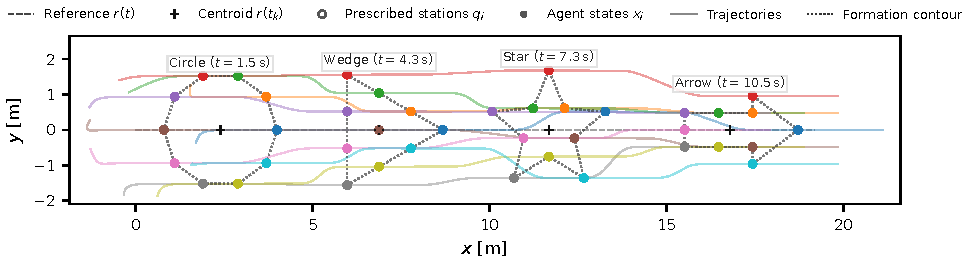
\includegraphics[width=0.98\linewidth]{figures/formation_snapshots.pdf}
\caption{Tracking sequential formation reconfigurations along a straight-line reference trajectory ($n=10$, $m=2.0$). Target formations (Hexagon at $t=1.5$~s, Wedge at $t=4.3$~s, Star at $t=7.3$~s, Arrow at $t=10.5$~s) are depicted with dashed contours, assigned target stations $q_i$ (circles), agent positions $x_i$ (dots), and continuous trajectories.}
\label{fig:reconfiguration}
\end{figure*}

\subsection{Finite-Time Tracking and Coupling-Gain Sweep}
Under rotating star compression ($\kappa=2.0$), the influence of cooperative coupling is examined for $m \in \{0.0, 0.5, 2.0, 5.0, 10.0\}$. \Cref{fig:convergence} and \cref{tab:gain-sweep} display the station error, formation disagreement, and control effort. Across all runs, agents reach station tracking within the universal deadline $T \approx 1.3621$~s, empirically verifying that exact finite-time convergence is independent of coupling gain and network topology. Concurrently, cooperative feedback accelerates convergence: settling times decrease monotonically with $m$ while maintaining moderate control effort.

\begin{table}[t]
\centering
\caption{Settling times and control effort across coupling gains $m$ under rotating star formation ($\kappa=2.0$, $T=1.3621$~s).}
\label{tab:gain-sweep}
\small
\begin{tabular}{ccccc}
\toprule
$m$ & $t_{10^{-6}}$ (s) & $T$ (s) & Peak $\norm{u}_2$ & $J_u$\\
\midrule
 0.0 & 1.1517 & 1.3621 & 16.9828 & 429.44 \\
 0.5 & 0.8117 & 1.3621 & 17.0860 & 429.92 \\
 2.0 & 0.5250 & 1.3621 & 18.0322 & 431.55 \\
 5.0 & 0.4467 & 1.3621 & 22.2186 & 434.95 \\
10.0 & 0.3933 & 1.3621 & 32.8156 & 440.74 \\
\bottomrule
\end{tabular}
\end{table}

\begin{figure*}[t]
\centering
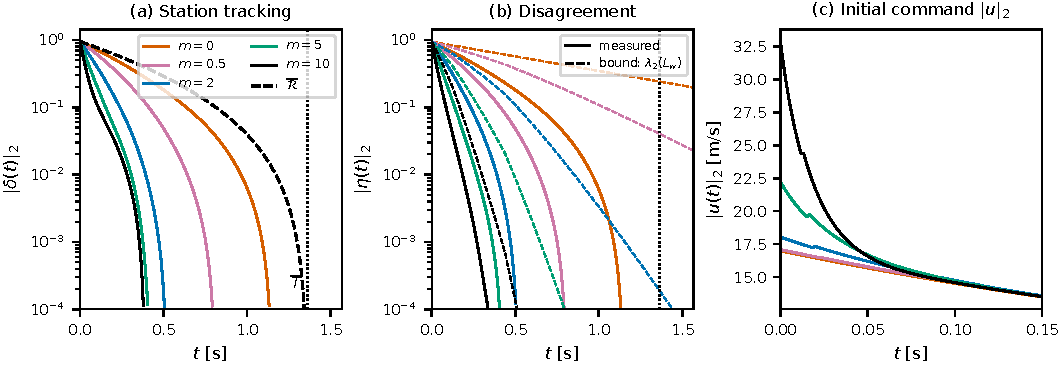
\includegraphics[width=0.98\linewidth]{figures/error_disagreement_control.pdf}
\caption{Finite-time tracking, disagreement decay, and initial control effort across coupling gains $m$ ($\kappa=2.0$). (a) Station tracking $\|\delta(t)\|_2$ against theoretical bound $\overline{\mathcal R}(t)$ and deadline $T$. (b) Disagreement $\|\eta(t)\|_2$ against analytical envelope bounds. (c) Transient control command $\|u(t)\|_2$ over $t \in [0, 0.15]$~s.}
\label{fig:convergence}
\end{figure*}

\subsection{Transient Safety and Collision Avoidance}
To highlight the necessity of cooperative coupling for collision prevention, Experiment~3 simulates aggressive compression ($a_0=1.70 \to a_\infty=0.72$ at $\kappa=5.0$), requiring $\gamreq = 4.4882$. The certified coupling gain $m=30.0$ ($\gamH=5.6194$) is benchmarked against uncoupled tracking $m=0.0$ ($\gamH=1.0$), with results summarized in \cref{tab:safety-comparison} and \cref{fig:safety-transient}.
For $m=30.0$, the theoretical condition $\gamH \ge \gamreq$ holds: the disagreement tube contracts within the prescribed geometric margin ($s(t) > \rho_{\mathcal{H}}(t)$), preserving inter-agent separation ($d_{x,\min} > \dsafe$) throughout the entire maneuver. Conversely, for uncoupled agents ($m=0.0$), independent tracking lag allows relative distortion to exceed the nominal clearance, producing an actual physical collision breach ($d_{x,\min} < \dsafe$) between $t=0.11$~s and $0.77$~s despite collision-free nominal stations.

\begin{table*}[t]
\centering
\caption{Transient safety and collision comparison under rapid star compression ($\kappa=5.0$, $t\in[0,2.5]$~s).}
\label{tab:safety-comparison}
\scriptsize
\begin{tabular}{lrrrrrrrrrl}
\toprule
Case & $m$ & $\kappa$ & $\gamH$ & $\gamreq$ & $t_{\mathrm{set}}$ (s) & $d_{x,\min}$ & $\ell_{x,\max}$ & Peak $\norm{u}_2$ & $J_u$ & Outcome\\
\midrule
Safe   & 30.0 & 5.0 & 5.6194 & 4.4882 & 0.3800 & 1.0326 & 4.0338 & 88.2953 & 513.97 & Certified; Safe, Connected \\
Unsafe &  0.0 & 5.0 & 1.0000 & 4.4882 & 1.1517 & 0.8605 & 4.0338 & 35.0544 & 480.66 & Uncertified; Safety Violation \\
\bottomrule
\end{tabular}
\end{table*}

\begin{figure*}[t]
\centering
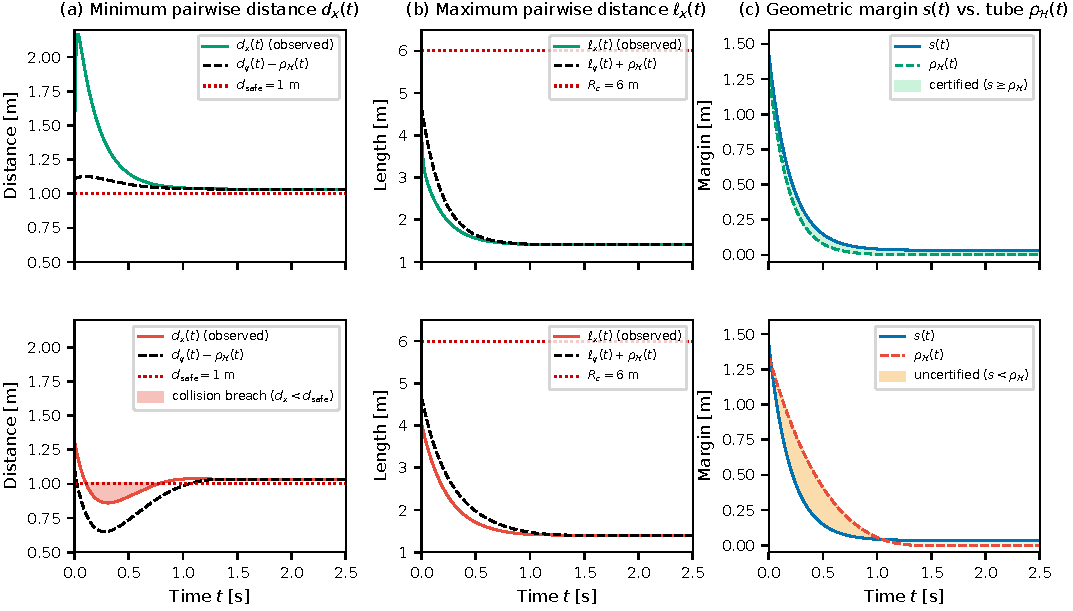
\includegraphics[width=0.98\linewidth]{figures/swarm_star_2x3_comparison.pdf}
\caption{Transient safety verification during fast star compression ($\kappa=5.0$, $t \in [0, 2.5]$~s). Top row: Certified Safe ($m=30.0$). Bottom row: Unsafe Mid-Transient Collision ($m=0.0$). Columns display minimum pairwise separation $d_x(t)$ (left), maximum pairwise distance $\ell_x(t)$ (middle), and geometric margin $s(t)$ versus disagreement tube $\rhoH(t)$ (right).}
\label{fig:safety-transient}
\end{figure*}

\subsection{Dual Expansion Maneuver and Connectivity Preservation}
The dual physical requirement---maintaining communication connectivity ($\ell_x(t) \le \Rc$)---is evaluated under rapid star expansion ($a_0=1.70 \to a_\infty=3.02$ at $\kappa=8.0$, $\gamreq=4.1367$), leaving a terminal clearance margin of merely $0.112$~m along the backbone. As reported in \cref{tab:expansion-comparison} and \cref{fig:expansion-transient}, the certified controller ($m=25.0$, $\gamH=4.8495$) coordinates agent expansion, bounding backbone edges safely below the communication threshold ($\ell_{x,\max} < \Rc$). In contrast, uncoupled agents ($m=0.0$) suffer substantial outward lag, causing severe network disconnection ($\ell_{x,\max} > \Rc$) for over $0.45$~s. Cooperative coupling is therefore indispensable for enforcing both transient safety and connectivity during aggressive swarming maneuvers.

\begin{table*}[t]
\centering
\caption{Transient connectivity preservation under rapid star expansion ($\kappa=8.0$, $t\in[0,2.5]$~s).}
\label{tab:expansion-comparison}
\scriptsize
\begin{tabular}{lrrrrrrrrrl}
\toprule
Case & $m$ & $\kappa$ & $\gamH$ & $\gamreq$ & $t_{\mathrm{set}}$ (s) & $d_{x,\min}$ & $\ell_{x,\max}$ & Peak $\norm{u}_2$ & $J_u$ & Outcome\\
\midrule
Safe   & 25.0 & 8.0 & 4.8495 & 4.1367 & 0.4183 & 1.8550 & 5.8880 & 83.5699 & 3624.11 & Certified; Safe, Connected \\
Unsafe &  0.0 & 8.0 & 1.0000 & 4.1367 & 1.1333 & 1.8550 & 6.1424 & 72.3516 & 3620.46 & Uncertified; Connectivity Violation \\
\bottomrule
\end{tabular}
\end{table*}

\begin{figure*}[t]
\centering
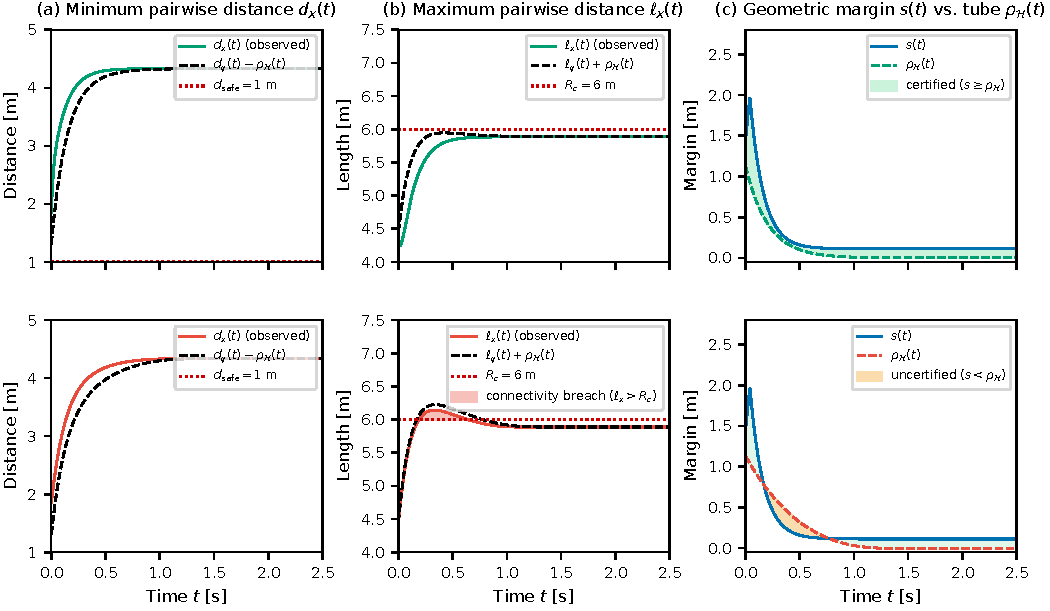
\includegraphics[width=0.98\linewidth]{figures/swarm_star_expansion_2x3_comparison.pdf}
\caption{Transient connectivity verification during fast star expansion ($a_0 = 1.70 \to a_\infty = 3.02$, $\kappa=8.0$, $t \in [0, 2.5]$~s). Top row: Certified Safe \& Connected ($m=25.0$). Bottom row: Unsafe Transient Disconnection ($m=0.0$). Columns display minimum pairwise separation $d_x(t)$ (left), maximum pairwise distance $\ell_x(t)$ (middle), and geometric margin $s(t)$ versus disagreement tube $\rhoH(t)$ (right).}
\label{fig:expansion-transient}
\end{figure*}

\section{Discussion and Limitations}
\label{sec:discussion}
The results separate three questions. First, assigned-station convergence is guaranteed in finite time independently of connectivity. Second, disagreement has an exponentially decaying upper bound that improves with the algebraic connectivity and the smallest eigenvalue of $M$. Third, safety and connectivity follow only when the planned station geometry leaves enough margin for that disagreement tube, including at the initial time. The third result is sufficient but conservative; a failed margin test is inconclusive rather than evidence of a collision.

The gain rule assumes access to the initial disagreement and to the geometry of the planned stations over $[t_0,T]$. It can therefore be used as an offline feasibility and gain-selection test, while the feedback itself uses assigned-station feedforward and neighbor-relative data. The model assumes first-order kinematics, exact reference/station feedforward, undirected interactions, symmetric positive-semidefinite $M$, and ideal continuous-time execution. Future work should include bounded disturbances, actuator limits, nonholonomic or second-order dynamics, localization uncertainty, and online replanning when the prescribed geometric margin becomes too small. A practical validation should also include at least one multi-agent initialization for which $\rho_0<s(t_0)$ and then verify the predicted sufficient-gain boundary against the measured trajectories.

\section{Conclusion}
A first-order distributed controller has been presented for exact finite-time tracking of arbitrary prescribed station trajectories. With centered offsets, the swarm centroid reaches its reference and the requested relative formation is recovered by the same finite-time deadline. An additional disagreement estimate provides a tube around the prescribed pairwise distances. For a connected spanning backbone, this tube yields sufficient safety and communication-range conditions and a closed-form inequality for selecting the coupling gain. The simulations show that coupling can reduce transient formation distortion and that nominally safe target stations alone do not prevent transient collisions. They also expose the conservatism of the certificate for the reported ten-agent initialization, motivating experiments designed explicitly to satisfy the initial-margin condition.

\bibliographystyle{IEEEtran}
\bibliography{references}
\end{document}